\documentclass[a4paper]{report}

%%%% Manual variants (JA or AJS)
\usepackage{etoolbox}
\newbool{AJS}
% Change this for different manual versions.
\setbool{AJS}{false}
% Shortcut commands
\newcommand{\AJSonly}[1]{\ifbool{AJS}{#1}{}}
\newcommand{\JAonly}[1]{\ifbool{AJS}{}{#1}}
\newcommand{\variant}{\ifbool{AJS}{AJS 37}{JA 37D}}

\newcommand{\versionnumber}{4.319}


% Todos:
% features.txt in the root directory

\usepackage[english]{babel}
\usepackage[utf8]{inputenc}
\usepackage[T1]{fontenc}
\usepackage{menukeys}
\usepackage{graphicx}
\usepackage{hyperref}
\usepackage{wallpaper}
\usepackage{xcolor}
\usepackage{geometry}
\usepackage{pdflscape}
\usepackage{gensymb}
\usepackage{multicol}
\usepackage{enumitem}

\usepackage{titlesec}
\titleformat{\chapter}[hang]{\bfseries\Huge}{\chaptertitlename\space\thechapter{}:}{1ex minus .1ex}{}
\titlespacing{\chapter}{0pt}{*0}{*3}

\pagestyle{headings}

\setcounter{tocdepth}{1}


\begin{document}
\newgeometry{bottom=2cm}
\ThisCenterWallPaper{1.0}{images/title}
\begin{titlepage}
  \centering
  \sf
  {\Huge Saab \variant{} Viggen}
  \\[1cm]
  {\Huge FlightGear Flight Manual}
  \\[16cm]
  \color{white}
  \emph{Model by}\\
  Anders Lejczak, Justin Nicholson, Enrico Castaldi,\\
  Joshua Davidson, Nicola B.\ Bernardelli, Isaac Protiva,\\
  Colin Geniet, Nikolai V.\ Chr.\\[0.2cm]
  \emph{Manual by}\\
  Colin Geniet, Rick Gruber-Riemer\\[1cm]
  Version \versionnumber{}
\end{titlepage}
\restoregeometry

\currentpdfbookmark{contents}{Contents}
\tableofcontents

\chapter*{Introduction}
\currentpdfbookmark{introduction}{Introduction}
\addcontentsline{toc}{chapter}{Introduction}

\section*{The Saab 37 Viggen}
The Saab 37 Viggen is a Swedish, supersonic, single-seat military aircraft,
notable for its short takeoff and landing capability offered by a thrust reverser.
It was developed in the 1960's, entered service in 1971, and was retired in 2005.
While the Viggen was intended as a multi-role aircraft,
it never truly achieved that goal---unlike its successor the JAS 39 Gripen.
Instead, the Viggen was developed into a multitude of versions for different roles:
surface attack (AJ 37), reconnaissance (SF 37, SH 37), and fighter interceptor (JA 37).

\subsubsection*{Specification (JA 37)}
\begin{tabular}{l@{\hspace{2cm}}l}
  Wing span                               & 10.60m \\
  Length                                  & 16.40m \\
  Height                                  & 5.93m \\
  Main wing area                          & 46.00m$^2$ \\
  Max takeoff weight                      & ca. 20000kg \\
  Max static thrust                       & 66.6kN dry, 110.3kN with afterburner \\
\end{tabular}

\section*{FlightGear Model}
This flight manual is intended for the Saab 37 Viggen model
for the \href{http://www.flightgear.org}{FlightGear} flight simulator.
The model is available through FlightGear's official hangar
\href{http://wiki.flightgear.org/FGAddon}{FGAddon}.
Alternatively, development versions can be found in the Github repository%
\footnote{\url{https://github.com/NikolaiVChr/flightgear-saab-ja-37-viggen}}.
Two variants of the Viggen have been developed in this model:
\begin{description}
  \item[JA 37D] A modernised fighter interceptor version from the 1990's.
    It notably features some of the glass instrument panels used in the JAS 39 Gripen.
  \item[AJS 37] Primarily a surface attack version,
    which resulted out of a modification programme providing some existing Viggens
    with limited multi-role (attack, fighter, and reconnaissance) capabilities.
\end{description}
This version of the manual is for the \variant{}.

\paragraph*{Compatibility Note}
This manual was designed for version \versionnumber{} of the Viggen model.
Minimum supported FlightGear version is 2018.3.x.
Using the latest stable FlightGear version is generally recommended.


\part{Aircraft Presentation}
\chapter{Cockpit Overview}

\begin{figure}
  \centering
  \includegraphics[width=\textwidth]{\ifbool{AJS}{images/panels/AJS-front-panel}{images/panels/JA-front-panel}}

  \begin{multicols}{2}
    \begin{enumerate}[nosep]
      \item Thrust reverser status light
      \item Thrust reverser handle
    \ifbool{AJS}{
      \item Autopilot pushbuttons/lights
      \item Autothrottle lights
      \item Airspeed/Mach indicator
      \item Radio frequency selector
      \item Angle of attack indicator
      \item Master warning lights and button
      \item HUD brightness knobs
      \item Attitude/director indicator (ADI)
      \item Altimeter
      \item Central indicator (CI)
    }{
      \item Backup attitude indicator
      \item Altimeter
      \item Backup altimeter
      \item Autopilot pushbuttons/lights
      \item G-meter
      \item Master warning lights and button
      \item Angle of attack indicator
      \item Autothrottle lights
      \item Airspeed/Mach indicator
      \item Afterburner zone lights
      \item Attitude/director indicator (ADI)
      \item RPM indicator (N2)
      \item Engine pressure ratio indicator
      \item HUD brightness knobs
      \item Target display (MI)
    }
      \item Parking brake handle
    \ifbool{AJS}{
      \item Clock
      \item HUD settings switches
      \item Backup attitude indicator
      \item Backup altimeter
      \item Backup heading indicator
      \item 'Weapon released' light
      \item G-meter
      \item Backup airspeed indicator
      \item RPM indicator (N2)
      \item Afterburner zone lights
      \item Engine pressure ratio indicator
      \item Transonic / low speed reverse light
      \item Waypoint type / number indicator
      \item Waypoint distance indicator
    }{
      \item Heading indicator
      \item Backup heading pushbutton/light
      \item Fast-reset pushbutton/light
      \item Transonic / low speed reverse light
      \item Horizontal situation display (TI)
    }
      \item Fuel gauge
      \item Left warning lights panel
      \item Right warning lights panel
    \end{enumerate}
  \end{multicols}

  \caption{Cockpit---front panel}
  \label{fig:front-panel}
\end{figure}

\begin{figure}
  \centering
  \includegraphics[width=\textwidth]{\ifbool{AJS}{images/panels/AJS-left-panel}{images/panels/JA-left-panel}}

  \begin{multicols}{2}
    \begin{enumerate}[nosep]
      \item Autothrottle lever
      \item Landing gear lever
      \item IR missile quick select
      \item Warning sounds volume
      \item Air conditioning controls
      \item Instruments light knob
      \item Panel light knob
      \item Backup trim controls
      \item Yaw trim centered light
      \item Trim reset button
      \item Radio control panel (not implemented)
      \item Canopy jettison button
      \item Radar control panel (not implemented)
    \AJSonly{\item Main mode selector knob}
      \item Engine start switch
      \item Generator switch
      \item Master power switch
      \item Fuel cutoff switch
    \JAonly{\item Radio channel selector KV3}
      \item Radio channel selector KV1 (not implemented)
      \item Warning lights test button
      \item Roll trim centered light
      \item Pitch trim indicator
      \item Brake pressure indicator
      \item Cabin pressure indicator
      \item Taxi/landing lights switch
    \end{enumerate}
  \end{multicols}

  \caption{Cockpit---left panel}
  \label{fig:left-panel}
\end{figure}

\begin{figure}
  \centering
  \includegraphics[width=\textwidth]{\ifbool{AJS}{images/panels/AJS-right-panel}{images/panels/JA-right-panel}}

  \begin{multicols}{2}
    \begin{enumerate}[nosep]
      \item Automatic fuel regulator switch
      \item Afterburner cutoff switch
      \item Emergency ram air turbine switch
      \item Pitch gearing switch
      \item Fuses panel
      \item ILS switch
      \item Weapons panel
      \item Countermeasures panel
      \item Manual fuel control switches
      \item Ignition plug switch
    \AJSonly{
      \item Nozzle position indicator
      \item Exhaust temperature indicator
    }
      \item Oxygen pressure indicator
      \item Oxygen cutoff switch
    \AJSonly{
      \item Radar altimeter switch
      \item DME switch---no functionality
    }
      \item Navigation panel
    \AJSonly{
      \item TILS channel selection knob
      \item TILS channel group switch
    }
    \JAonly{
      \item Radar altimeter switch
      \item GPWS switch
    }
      \item Windshield defogging knob
      \item Test panel
    \JAonly{
      \item Nozzle position indicator
      \item Exhaust temperature indicator
    }
      \item Data panel \AJSonly{(not implemented)}
      \item RWR control panel
    \JAonly{
      \item Navigation radio panel
    }
      \item Transponder
      \item Formation lights switch
      \item Navigation lights switch
      \item Anti-collision lights switch
      \item Identification transponder panel
      \item Formation lights intensity knob
    \end{enumerate}
  \end{multicols}

  \caption{Cockpit---right panel}
  \label{fig:right-panel}
\end{figure}



\chapter{Instrumentation}
\chapter{Systems}
% TODO: https://github.com/NikolaiVChr/flightgear-saab-ja-37-viggen/issues/120
%\section{Course Correction for Magnetic Deviation}
%Like in the real Viggen there are two ways to set the course correction, which makes sure that the instruments show true North instead of magnetic North (e.g. in north Norway the deviation is larger than 12\degree):
%\begin{itemize}
% \item Automatic: Simplified the computer averages the deviation between measured between 110 and 200 km/h during take-off.
% \item Manual: Make sure your airplane is properly aligned with the runway. Press FIXME. The reason for doing it manually is if the runway is slippery or there are strong crosswinds, which might change the way the nose points and therefore give a wrong deviation measurement. 
%\end{itemize}

%Please note that the computer in the real Viggen also makes some comparisons with the stored runway heading(s) to decrease the risk of failures. Warning light \emph{NAV SYST} would lit up. However, this is not modelled in FlightGear. 

%\AJSonly{Reference: [AJS\_1, sec. 20, ch. 3.4, p. 312]}

\part{Flight Operation}
\chapter{Generic FlightGear Operations}
\section{Menu Entries and In-Flight Configuration}
\subsection{Menu Help}
The Help menu contains 2 menu items, which are Viggen specific:
\begin{itemize}
\item Aircraft Help: the top section contains the most important key bindings for the Viggen\footnote{The displayed list is only a selection. For the total list you need to delve into the installation directory and look into \directory{flightgear-saab-ja-37-viggen/Aircraft/JA37/Systems/ja37-input.xml}.}. The lower section contains a set of tips to get your started with flying.
\item Aircraft Checklists: A set of interactive checklists especially for start-up, taxi, take-off and landing.
\end{itemize}

\subsection{Menu AJS-37}
This menu contains a set of menu items, which ease some configurations, which are not available otherwise or would be tedious to do.
\begin{itemize}
\item Select Livery: there is a variety of liveries available, some of which are fictional. Note that the dialog does not take care of whether a livery belongs to the AJS or JA Di version: if you want to fly authentic, you need to know yourself.
\item Auto start/stop: Lets you start and stop the plane without needing to switch switches etc. yourself. The progress is shown in the top centre of the screen in blue text. \glqq Engine ready\grqq is the final notification of the start-up sequence. The shut-down sequence is done, when the aircraft is dark.
\item Repair: repairs system failures etc. when you are on the ground. If you have crashed, then there is no help.
\item Fuel/Loadout: Opens a custom dialog to allow fast selection of a suitable loadout and fuel settings. This is an alternative to menu item Fuel and Payload in menu Equipment. It will make sure that you only select weapon combinations, which were valid in the real Viggen.

\begin{figure}[h]
\centering
 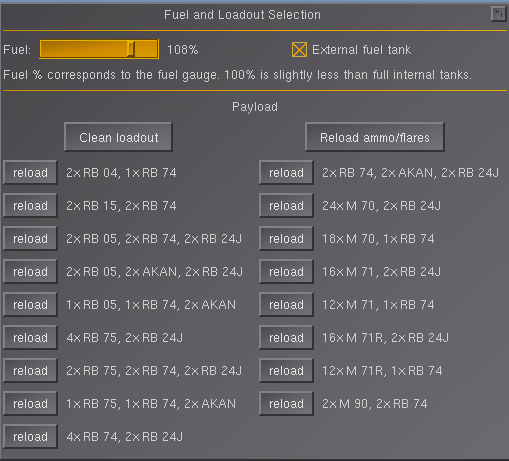
\includegraphics[width=10cm]{images/fg_loadout_dialog.png}
 \caption{Viggen specific fuel and loadout selection dialog}
\end{figure}

\item Performance Monitor: shows performance values, some of which are also available on original instruments (mostly for developers)
\item Systems Monitor: ditto for systems (mostly for developers)
\item Toggle external power: note that this is one of the things added and removed automatically when using the auto start/stop function.
\item Options: various configuration options. Note that the Viggen was a Swedish fighter and therefore the most authentic settings are with Swedish labels and for the AJS with metric instead of imperial units.
\end{itemize}

\begin{figure}[h]
\centering
 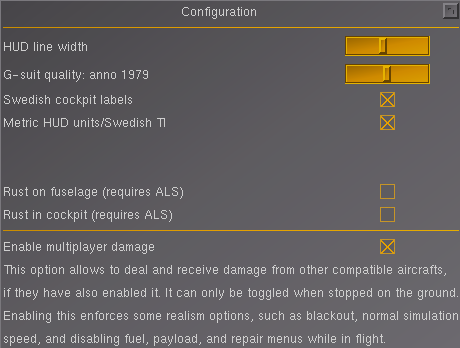
\includegraphics[width=10cm]{images/fg_option_config.png}
 \caption{Viggen specific options dialog}
\end{figure}


\chapter{Standard Procedures}
\chapter{Emergency Procedures}
\chapter{Miscellaneous Notes}
\section{JA 37Di Related}
Be mindful of failure messages in the TI display FAIL menu, if a gear locking mechanism fails due to being deployed at too high speed, that gear will not be able to support the weight of the aircraft till you repair it from the menu.

\part{Weapons Operation}

\chapter{Ground and Naval Attack}
\AJSonly{
\section{Rb 05A missile}
\label{Rb05A}
\begin{figure}[h]
\centering
 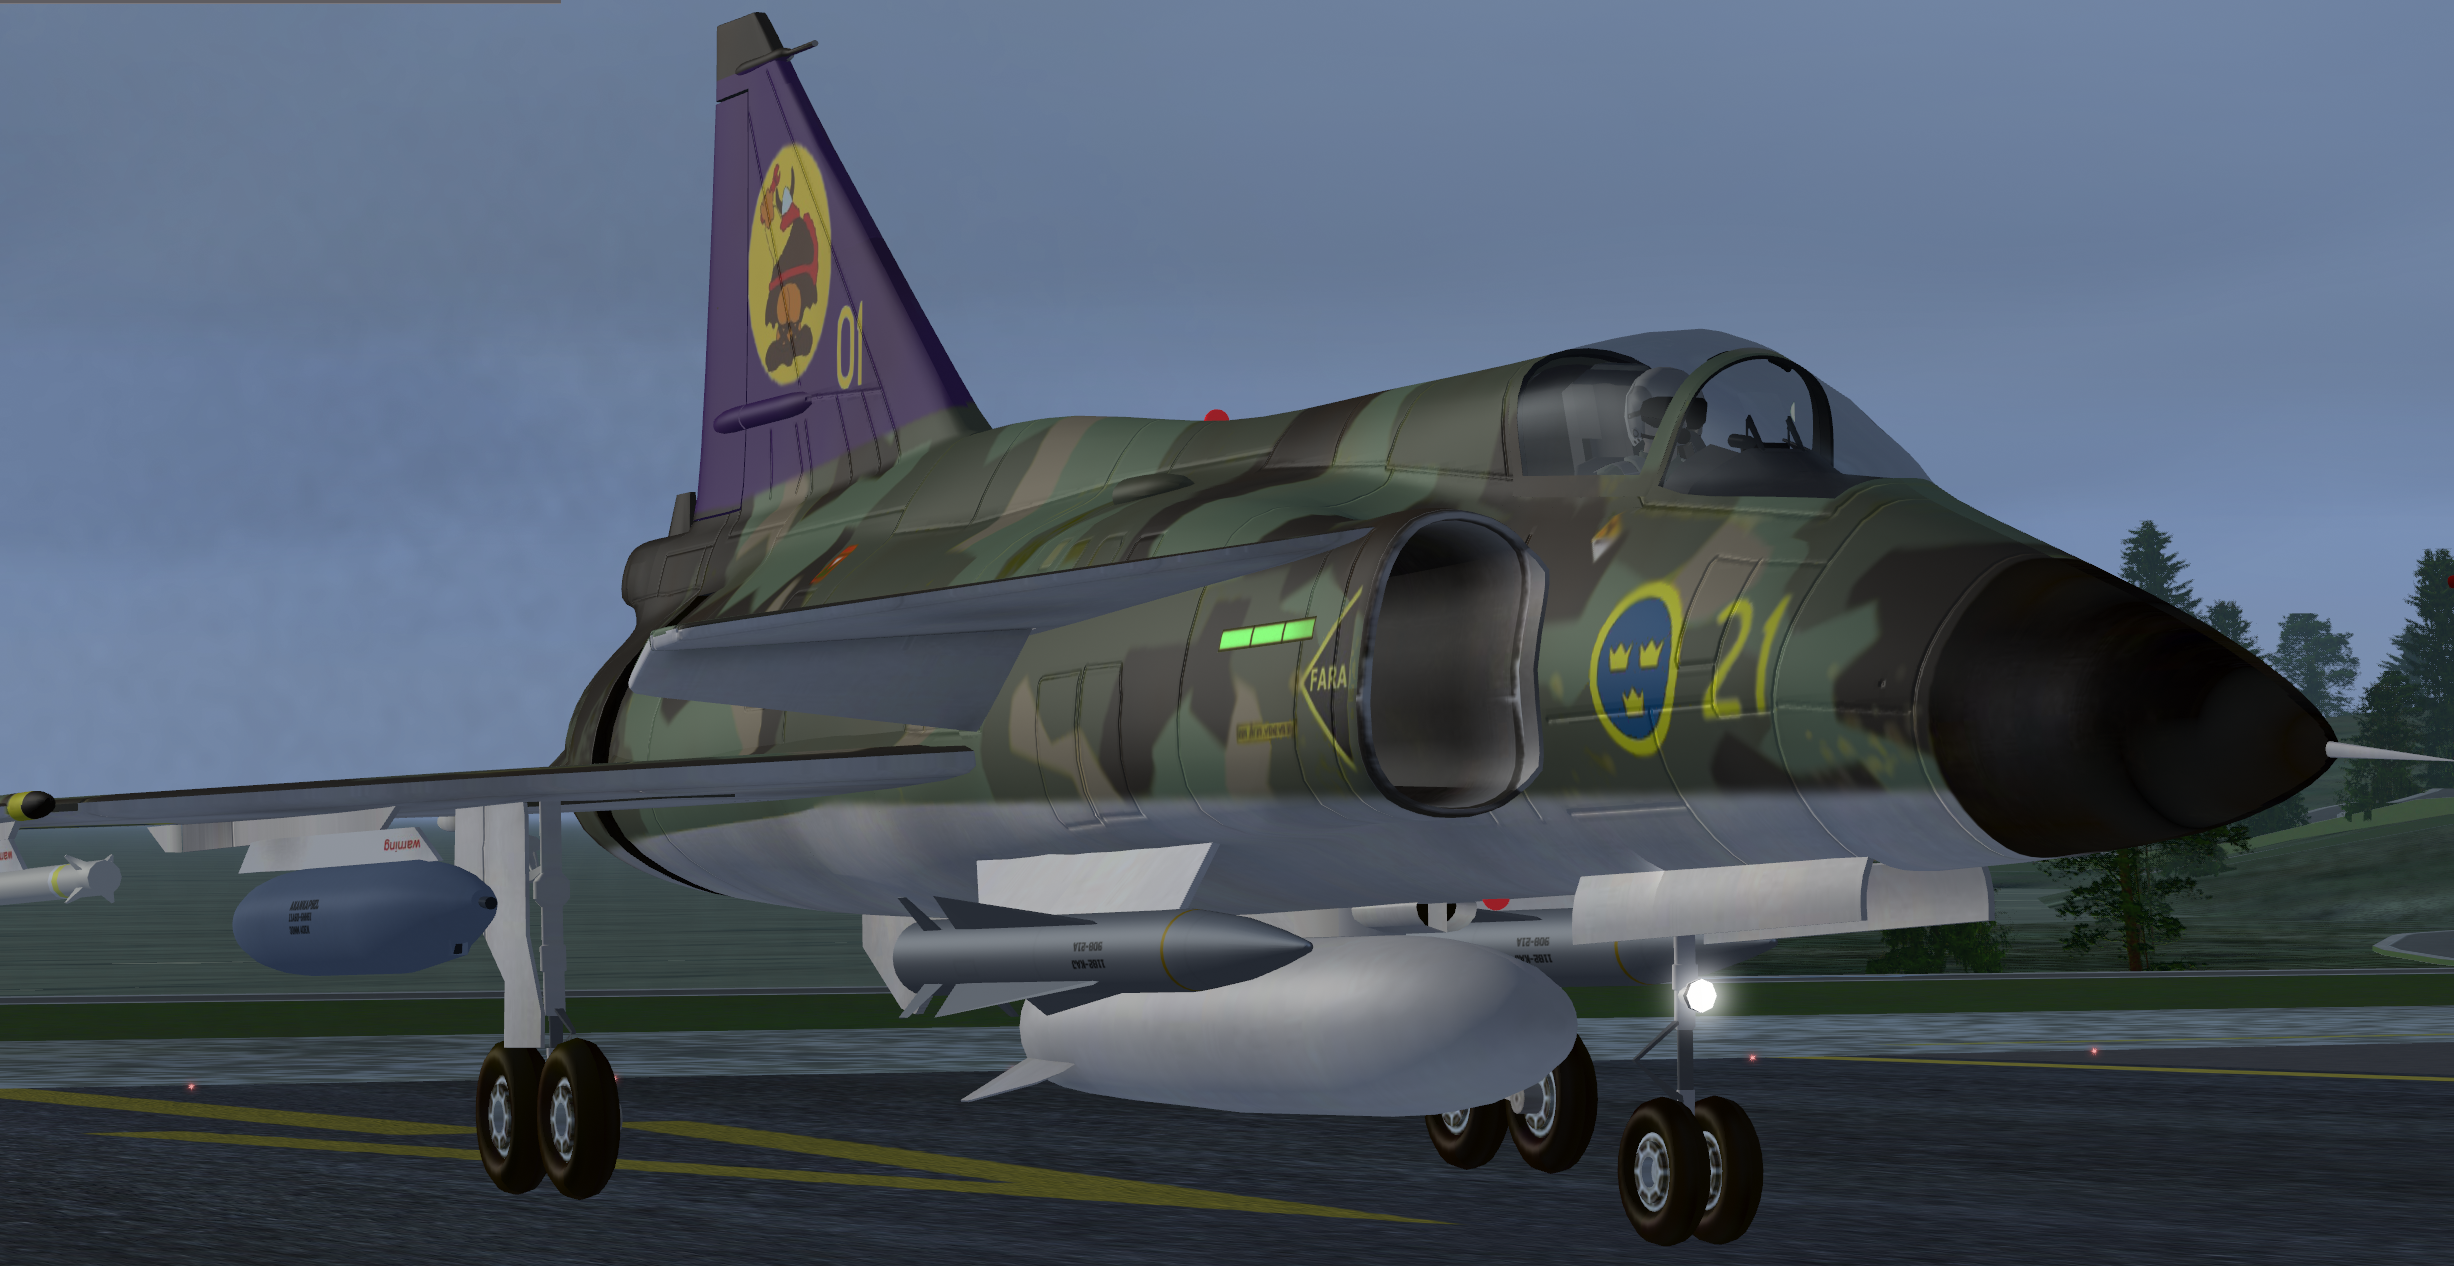
\includegraphics[width=15cm]{images/rb_05a_load_with_akan.png}
 \caption{AJS 37 with 2 Rb 05A on the inner pylons}
\end{figure}

The Rb 05A was a jam-proof, radio guided super-sonic missile developed in Sweden with similar characteristics as the AGM-65 Maverick. While an optical/IR guidance system was planned, it never got realised because the Maverick was adapted as the Rb 75 instead. The missile was constructed for use against ground and naval targets, but later it was discovered that it could also be used against slow-manoeuvring air targets. 

As the missile was guided visually by the pilot, a smoke free propellant was used and there was a flare in the back. During the first 1.7 seconds of the missile's flight, it was auto guided to fly into the pilot's visual field in front of the aircraft's nose.

\begin{figure}[h]
\centering
 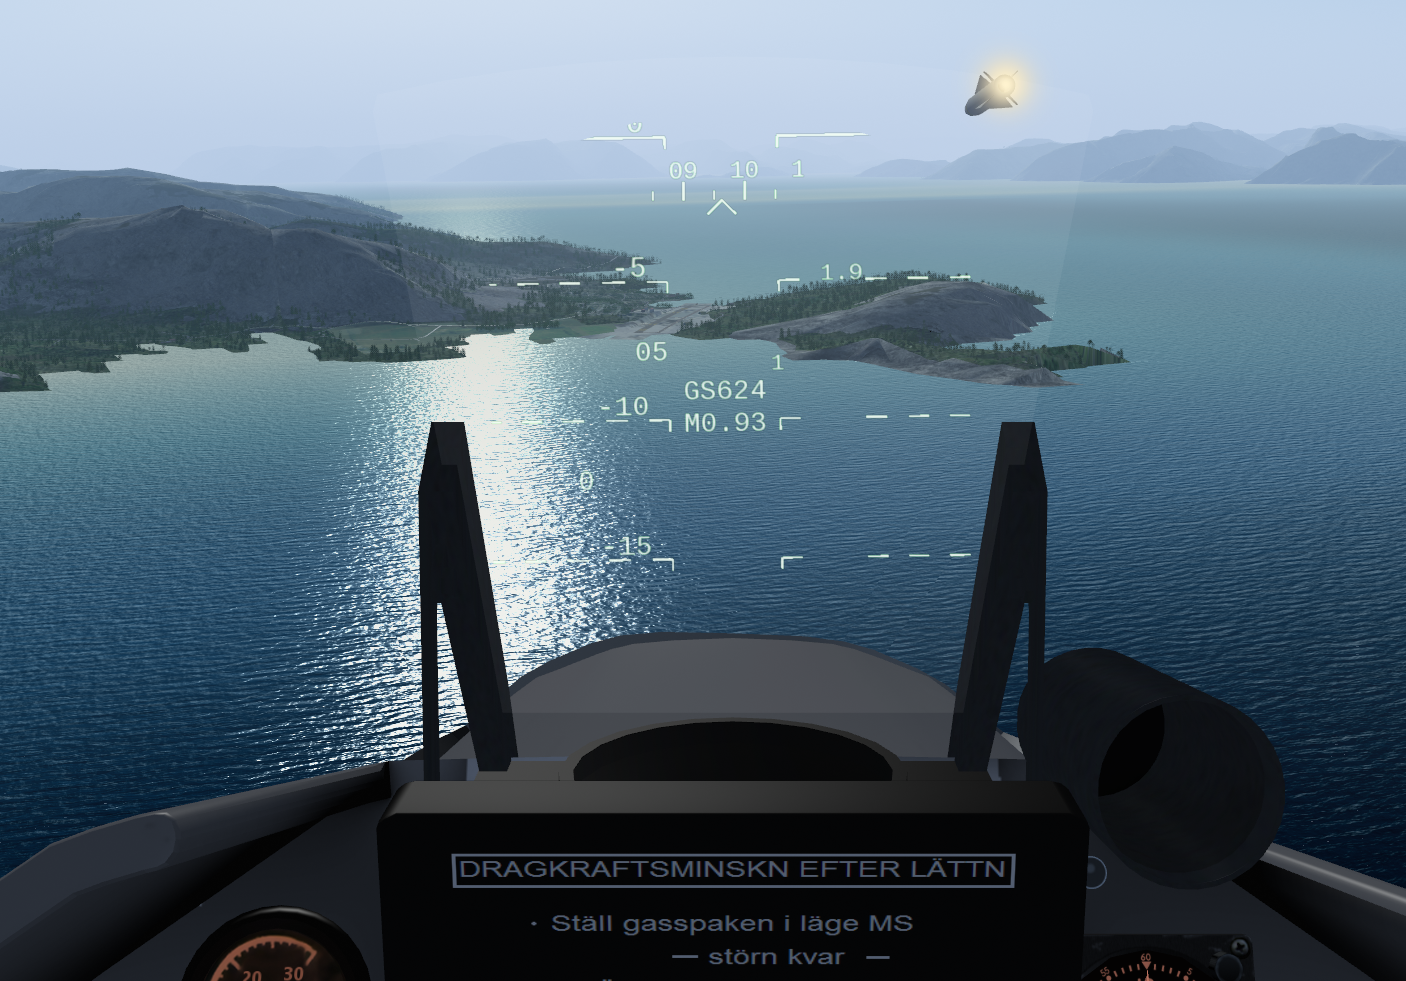
\includegraphics[width=10cm]{images/rb_05a_start_popup.png}
 \caption{The Rb 05A is guided automatically into the pilot's view just after the launch.}
\end{figure}

To manually guide the missile in the real Viggen, a mini-joystick on the right console was used with the right hand. Therefore, one of the following was used to free the right hand from the stick:
\begin{itemize}
 \item Take the stick with the left hand and fly the airplane. Reference: [AJS\_2, ch. II, p. 86]
 \item If missile guidance is done during the aircraft flying horizontal, then use autopilot for altitude. If it is done during a light dive, use autopilot for attitude. Reference: [AJS\_3, sec. 7, ch. 5, p. 210]
\end{itemize}

On page 25 in issue 4/1972 of the Swedish magazine \href{https://www.aef.se/Flygvapnet/Tidskrifter/FV_Nytt/Flygvapennytt_1972-4.pdf}{FlygvapenNytt} there is a good description of the capabilities and evolution of the weapon.

Operations (reference: [AJS\_3, sec. 7, ch. 5, p. 210] for description, [AJS\_2, ch. II, p. 86] for procedure):
\begin{enumerate}
 \item Fly fast and low, navigate to the pre-programmed pop-up point in \emph{NAV} mode.
 \item Before reaching the pop-up point:
 \begin{itemize}
  \item Correct the atmospheric pressure.
  \item Choose mode \emph{ANF}.
  \item Set the \emph{J/A} weapons knob to Rb 05A with the correct fuse (MARK for ground, SJÖ for naval). Not yet modelled correctly in FlightGear: instead choose the Rb 05A by pressing \keys{w} until displayed on the HUD.
  \item Check that the autopilot is on \emph{SPAK} only.
 \end{itemize}
 \item A fast pop-up is done to 300--400 metres above ground at the pre-programmed pop-up point --- either with pitch only or in a half roll.
 \item Identify the target and fly level or slightly downwards. The nose does not have to point to the target. 
 \item Consider engaging the \emph{ATT} or \emph{ALT} autopilot mode.
 \item Fire within 9 km of the target at a speed between 700 km/h and 1150 km/h.
 \item Guide the missile visually using the collimation principle --- to begin with roughly and then more and more accurate until the missile' flare covers the target.
 \item When the missile has hit the target, evade as quickly as possible and choose \emph{NAV} mode.
\end{enumerate}

\begin{figure}[h]
\centering
 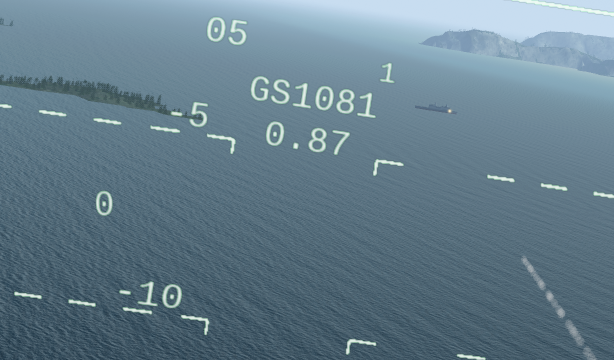
\includegraphics[width=10cm]{images/rb_05a_before_impact_ship.png}
 \caption[Flare at back of missile for guidance]{The flare at the back of the missile is used for visual guidance. Here it can be seen just moments before hitting the ship --- clearly off the bore sight and flight path of the aircraft.}
\end{figure}

Operations in FlightGear:
\begin{itemize}
 \item There is no need to lock the target. There is no functionality to set the trigger to unsafe\footnote{In the real Viggen a battery would be activated and the missile would have to be shot within 40 seconds or it would get unusable.}. And there is no specific HUD mode (as in the real Viggen).

 \item Fire with the trigger.
 \item Guide the missile by using one of the following methods:
 \begin{itemize}
  \item Use the keybinding \keys{y} to toggle the joystick to be a cursor and then use the usual axis to guide the missile. Note: needs to be done after the trigger has been pressed. To be able to use the joystick for the flight controls again, you need to press \keys{y} again. If the ground collision warning is triggered, then the joystick is automatically set back to control the aircraft again, but you will have lost guidance on the missile.
  \item Bind the following to axis of your joystick or throttle: \textbf{\texttt{/controls/displays/cursor-slew-x}} and \textbf{\texttt{/controls/displays/cursor-slew-y}}. This makes it possible to have different sensitivity from the joystick. Note that it is the same binding as e.g. used in the JA 37Di variant --- but the AJS does not have a screen with a cursor (and the JA 37Di does not have the Rb 05A).
 \end{itemize}

\end{itemize}

Tips:
\begin{itemize}
 \item Make sure to fly within the recommended speed of 700 km/h--1150 km/h. You might loose sight of the light at the back of the missile and would probably not be able to see the target anyway.
 \item The missile flies for ca. 24 seconds. The max. distance of 9 km can only be reached if the flight path is relatively straight and the aircraft's speed at launch is within the recommended parameters. Therefore, the missile might explode after 24 seconds before it reaches the target, e.g. if the steering commands by the pilot make it swing a lot and thereby loose speed. See also [AJ\_2, ch. 1:6, figure 51, p. 64].
 \item Make sure to fly either straight horizontal or in a light dive. If you have your nose up, you might loose track of the missile and/or target. Note that one of the advantages of this missile is that it can be guided considerable off bore sight.
 \item Especially for large objects (factory) make sure to aim in the middle of the object and on ground level. The proximity fuse might otherwise not recognise it.
 \item Turn off the radar \keys{r} to reduce clutter in the HUD by target symbols.
\end{itemize}

}

\chapter{Air to Air}
\AJSonly{
\section{Rb 05A missile}
The Rb 05A could also be used against slow flying air targets like helicopters or transport planes. See section \ref{Rb05A} on page \pageref{Rb05A} for a description. The difference to ground/naval attack is that the distance had to be measured with the radar.

}

\section{Cannon}
\url{https://www.aef.se/Flygvapnet/Tidskrifter/FV_Nytt/Flygvapennytt_1993-2.pdf} has an article and 2 pictures about the automatic aiming mode for the cannon in the JA version (in Swedish).

\appendix

\chapter{References}

A comprehensive book in English covering all variants is \glqq Saab 37 Viggen --- The ultimate portfolio\grqq by Jan Jørgensen (published in 2014 by \href{http://www.nordicairpower.com/}{Nordic Airpower}).

\subsection{Original Manuals}
A significant part of the original manuals are available on the internet, and in recent years also many of the formerly classified chapters (as far as the information is not still valid due to (re-)use in the Gripen) have been become available. As the Viggen could not be sold to other countries\footnote{Austrian pilots went through a training programme on the Viggen to familiarise with modern combat airplane, but never bought it}, a significant part of the text and illustrations are in Swedish.

The following manuals are core to the understanding of flying a Viggen in military operations. Where possible, references are made in this manual to text elements in the original manuals(e.g. [AJS\_Del1, sec. 20, ch. 3.4.2, p. 312]). Also, this manual does typically not repeat illustrations from the original handbooks, but shows a screenshot from the simulation instead, so you can compare.

\begin{table}[!th]
\begin{tabular}{|l|l|c|r|}
\hline
Ref & Title & Date & Pages \\
\hline
AJ\_Del2 & FPL AJ37 Speciell Förarinstruktion Del 2 kap 1 (M5800--370011) & 1975--02--01 & 181 \\
AJS\_Del1 & FPL AJS37 Speciell Förarinstruktion Del 1 (M5800--370011) & 1994--11--15 & 517 \\
AJS\_Del2 & FPL AJS37 Speciell Förarinstruktion Del 2 (M5800--370011) & 1994--11--01 & 222 \\
AJS\_Del3 & FPL AJS37 Speciell Förarinstruktion Del 3 (M5800--370011) & 1994--11--15 & 295 \\
JA\_Vol1 & Flight Manual A/C JA37 Volume 1 (M5800-370051) & 1999--01--20 & 497 \\
\hline
\end{tabular}
\caption{Overview of flight manuals from the original Viggen}
\end{table}

\subsection{FlightGear Related}
\begin{itemize}
\item The \href{http://wiki.flightgear.org/Saab_37_Viggen}{FG wiki article} contains a comprehensive feature overview, links to forum articles etc. However, the wiki is not always up to date.
\item \href{http://opredflag.com/}{Operation Red Flag (OPRF)} is a FlightGear military simulation community discussing, developing and using many of the combat features in the Viggen.
\item On Discord there is a dedicated \href{https://discord.gg/jc5pSM5}{Viggen server} and a \href{https://discord.gg/SmGFnJN}{OPRF server}. Say hello and discuss the Viggen's features, development and your flight experience. Preliminary help with issues can be gotten as well, confirmed issues should be reported in the Viggen's \href{https://github.com/NikolaiVChr/flightgear-saab-ja-37-viggen/issues}{issue tracker} for resolution.
\item The \href{https://www.youtube.com/playlist?list=PLogi97V-ki0GfCLqimTtIq9RIVcm-GRFE}{Flightgear Saab 37 Viggen YouTube Playlist} includes amongst others a set of tutorial videos featuring the JA and the AJS variant.
\end{itemize}

\subsection{Other Combat Flight Simulators}
Both \href{https://www.digitalcombatsimulator.com/en/index.php}{DCS} and \href{https://www.benchmarksims.org/}{BMS Falcon} have flyable Viggens. Especially for DCS there is an abundance of resources available on the internet (e.g. YouTube). Please note that while there can be valuable additional information and context provided in content from other simulators, the capabilities modelled will differ.

\subsection{Swedish Documentation Sites}
\begin{itemize}
\item Arboga Elektronikhistoriska Förening: \url{https://www.aef.se}, e.g. 
\begin{itemize}
\item \href{https://www.aef.se/Avionik/Notiser/PS-37/PS-37A.htm}{Spanings- och siktesradar PS-37/A (for the AJS)}
\item \href{https://www.aef.se/Avionik/Notiser/Siktesradar_PS-46_1.htm}{Flygradarinstallation JA37 ---Siktesradar PS46} (includes links to 2 articles from Ericsson)
\item \href{https://www.aef.se/Flygvapnet/Tidskrifter/FV_Nytt/FVN_oversikt.htm}{FlygvapenNytt 1960 – 2003}: \url{https://www.aef.se/Flygvapnet/Tidskrifter/FV_Nytt/Flygvapennytt_1991-2.pdf} announced the AJS Viggen and \url{https://www.aef.se/Flygvapnet/Tidskrifter/FV_Nytt/Flygvapennytt_1994-4.pdf} had follow-up articles.
\end{itemize}
\item Digitalt Museum: \url{https://digitaltmuseum.se/}:
\begin{itemize}
\item Aeroseum Göteborg: \url{https://digitaltmuseum.se/owners/S-AER}
\item Flygvapenmuseum: \url{https://digitaltmuseum.se/owners/S-FV}
\item Teknikland: \url{https://digitaltmuseum.se/owners/S-TL}
\item Sveriges militärhistoriska arv: \url{https://digitaltmuseum.se/owners/S-MHA}
\end{itemize}
\end{itemize} 


\begin{landscape}
\chapter{Viggen Related Videos}
The following selection of videos has been made based on operational content or visibility of details. There exist many more videos --- some of which with higher quality from recent air shows. If you miss a video below, let us know.

\begin{table}[!th]
\begin{tabular}{|p{5cm}|c|c|c|p{9cm}|}
\hline
Title & Length & Subtitles & Year & Comments \\
\hline

\href{https://www.youtube.com/watch?v=kBq5qA8r4dA}{SF/SH37 \& JA37 VIGGEN at F13 Wing} & 18 min & yes & 2000 & Mostly about the reconnaissance and photo version\\
\href{https://www.youtube.com/watch?v=0sRACNVVmpE}{Saab 37 Viggen 2001 1-2} & 15 min & no & ?? & Historic part plus early versions\\
\href{https://www.youtube.com/watch?v=pAPteuBsRGg}{Saab 37 Viggen 2001 1-2} & 14 min & no & ?? & Mostly about the evolution of the JA. Some footage of HUD and CI/TI screens.\\
\href{https://www.youtube.com/watch?v=fmqXa0oetUA}{VI FLÖG HÅRT OCH STRIDSMÄSSIGT} & 15 min & no & ?? & A fighter pilot tells stories\\
\href{https://www.youtube.com/watch?v=ErK3zaNRccE&}{Jaktviggenpilot på Bråvallajakten} & 14 min & no & 1989 & A day in the live of a fighter pilot\\
\href{https://www.youtube.com/watch?v=qaNt9_sQdGI}{Kurvstrid (Dogfight) SAAB JA37C VIGGEN} & 8 min & yes & ?? & Various dogfights with some HUD visibility\\
\href{https://www.youtube.com/watch?v=oB6-jJEWjWk}{S som i Speed - Göran flyger Viggen} & 6 min & no & 1996 & Some low level flying\\
\href{https://www.youtube.com/watch?v=gwgJNdWZlj0}{SH-37 Viggen Sea Surveillance} & 4 min & n/a & ?? & Some nice sequences of the AJS CI and a few glipse of the HUD\\
\href{https://www.youtube.com/watch?v=mgPS5-SbI0c}{Viggen attackuppdrag} & 2 min & no & ?? & Attack with rockets using pop-up method. Some sequences of the HUD.\\
\href{https://www.youtube.com/watch?v=eQjAp7bTnUg}{Kalla Krigets Fordon avsnitt 6: SAAB 37 Viggen} & 9 min & no & 2016 & A bit of history and relation between the plane and the road base system. During the very last seconds some close-up sequences of the CI.\\
\href{https://www.youtube.com/watch?v=slm9ksxU0HY}{Viggen Road base exercise} & 6 min & n/a & ?? & As the title says.\\
\href{https://www.youtube.com/watch?v=hWrsP3hq5M8}{AJ-37 Viggen Low Level Flying} & 4 min & n/a & ?? & As the title says. Some HUD sequences incl. rocket attack.\\
\href{https://www.youtube.com/watch?v=UOszNlNeRVs}{SAAB 37 Viggen} & 4 min & n/a & ?? & Some nice air ballet plus a few sequences of the CI.\\
\href{https://www.youtube.com/watch?v=IbsYsUvCy7s}{Rörlig klargöring JA37 Arlanda} & 43 min & no & 1996 & Ground operations of JA 37 on an improvised stand at Arlanda airport\\
\href{https://vimeo.com/60091080}{Viggen i Älskar, älskar inte} & 4 min & no & ?? & Excerpts from the feature film, Älskar, älskar inte. Nice dogfighting between JA and AJS plus some CI sequences\\
\href{https://www.youtube.com/watch?v=eT00_OVrv7o}{JA-37 and SK-37E Night Ops} & 7 min & no & ?? & Night flying with good pictures of exhaust, navigation and beacon lights\\
\href{https://www.youtube.com/watch?v=0ocSUd9_5Tw}{JA37 F21 1982-2004} & 17 min & no & ?? & Around min 5 and 15 there are longer sequences of the HUD in weapons mode (JA variant)\\

\hline
\end{tabular}
\caption{Selected videos featuring the Viggen. Unless described otherwise in the comments, the language is Swedish}
\end{table}

% Videos watched but not found interesting enough
% \href{https://www.youtube.com/watch?v=rFZKvO95bQ0}{2018-10-17 Svensk stridspilot under det kalla kriget}
% \href{https://www.youtube.com/watch?v=RHVzkVwI68w}{Vetenskapens Värld - Viggen} Mostly project and politics history until first viggen operational
% \href{https://www.youtube.com/watch?v=M8HF1gH0MPc}{37 Viggen - The Power of Viggen!} Mostly flight display
% \href{https://www.youtube.com/watch?v=Z_EnkvE6LZA}{Fredens Hav}
\end{landscape}

\end{document}
